\documentclass[11pt,a4paper]{article}

\usepackage[utf8]{inputenc}
\usepackage[T1]{fontenc}
\usepackage{amsmath,amssymb,amsthm}
\usepackage{booktabs}
\usepackage{graphicx}
\usepackage[margin=1in]{geometry}
\usepackage{hyperref}
\usepackage{enumitem}
\usepackage{xcolor}
\usepackage{algorithm}
\usepackage{algpseudocode}
\usepackage{multirow}

\newtheorem{theorem}{Theorem}
\newtheorem{definition}{Definition}

\title{TAHOE: Task-Aware Language Harness for Orchestrated Execution}
\author{Anonymous}
\date{}

\begin{document}
\maketitle

\begin{abstract}
TAHOE is a structured reasoning language that teaches large language models (LLMs) to think in typed protocols---\textsc{Compute}, \textsc{Select}, \textsc{Deduce}---rather than free-form chain-of-thought.
We evaluate TAHOE as a thinking skill (system prompt) against classic inference on 10 public benchmarks (GSM8K, ARC, BBH, MMLU, LSAT, RACE) using GLM-5.3-Flash with 10 samples per benchmark, 3 trials per sample, 600 trials total.
Results show TAHOE improves pass rate by 1\% (89\% vs.\ 88\%) while reducing reasoning token consumption by 40\% (60{,}055 vs.\ 100{,}595 output tokens).
The harmonic mean of quality and efficiency is 1.162 (TAHOE) vs.\ 0.934 (classic), indicating TAHOE wins on both axes simultaneously.
We provide formal operational semantics for the language, a frozen evaluation protocol, and bootstrap confidence intervals for all reported metrics.
\end{abstract}

\section{Introduction}

LLM reasoning quality varies with problem structure.
Free-form chain-of-thought (CoT) prompting~\cite{wei2022cot} improves accuracy but produces verbose, unstructured output that wastes tokens.
As models are deployed at scale, the cost of reasoning tokens becomes a first-order concern: each redundant token increases latency, compute, and inference cost without improving answer quality.

TAHOE addresses this by providing a language for structured reasoning that the model applies internally as a \emph{thinking skill}---a system prompt that shapes how the model reasons without changing the task or the output format.
The key insight is that the system prompt (93 tokens) is a fixed infrastructure cost, while the model's reasoning (output tokens) is where TAHOE delivers value: structured reasoning is more compact than free-form narrative, producing 40\% fewer tokens while also improving accuracy.

\paragraph{Contributions.}
\begin{itemize}[nosep,leftmargin=*]
    \item \textbf{TAHOE language}: a typed, protocol-based reasoning language with formal operational semantics (Section~\ref{sec:language}).
    \item \textbf{Evaluation methodology}: a frozen evaluation protocol with rigorous token accounting and bootstrap confidence intervals (Section~\ref{sec:methodology}).
    \item \textbf{Empirical results}: 600-trial controlled experiment showing 40\% token reduction with 1\% quality improvement (Section~\ref{sec:results}).
    \item \textbf{Formal semantics}: small-step operational semantics with progress and preservation theorems (Section~\ref{subsec:formal}).
\end{itemize}

\section{TAHOE Language}
\label{sec:language}

TAHOE is a structured reasoning language that constrains LLM output into typed, protocol-governed patterns.
The language has three core components: typed refs, protocols, and a need-trigger mechanism.

\subsection{Typed Refs}
\label{subsec:typed-refs}

TAHOE distinguishes knowledge states using typed references (refs).
Each ref carries a type tag from a fixed vocabulary:

\begin{center}
\begin{tabular}{ll}
\toprule
\textbf{Type} & \textbf{Role} \\
\midrule
G & Goal \\
C & Constraint \\
E & Evidence \\
H & Hypothesis \\
U & Unknown \\
O & Option \\
K & Criteria \\
D & Decision \\
P & Result \\
V & Verified \\
OUT & Output \\
\bottomrule
\end{tabular}
\end{center}

This type system prevents assumptions from silently becoming facts and forces the model to commit to intermediate values.
The types form a subtyping lattice (Section~\ref{subsec:formal}) where stronger types (e.g., \texttt{V} for verified) can substitute for weaker ones (e.g., \texttt{H} for hypothesis) but not vice versa.

\subsection{Protocols}
\label{subsec:protocols}

Three core protocols map task types to reasoning patterns:

\begin{itemize}[nosep,leftmargin=*]
    \item \textbf{Compute}: $\texttt{E.givens} \to \text{steps with concrete numbers} \to \texttt{verify} \to \texttt{answer}$
    \item \textbf{Select}: $\texttt{O.options} \to \text{eliminate wrong} \to \texttt{D.pick} \to \texttt{answer}$
    \item \textbf{Deduce}: $\texttt{C.constraints} \to \text{assign positions explicitly } (1..N) \to \texttt{verify all} \to \texttt{answer}$
\end{itemize}

Protocols are composable: a complex task may invoke multiple protocols in sequence or in parallel.
Counterfactual reasoning, for instance, reduces to three existing commands---\texttt{hypothesize}, \texttt{challenge}, \texttt{verify}---without requiring new syntax.
The typed-ref system (\texttt{H.*} vs.\ \texttt{E.*} vs.\ \texttt{V.*}) enforces the distinction between counterfactual hypothesis, factual evidence, and verified verdict, preventing the silent substitution that Pearl's do-calculus was designed to expose~\cite{pearl2009causality}.

\subsection{Need-Trigger}
\label{subsec:need-trigger}

TAHOE is need-triggered: the model applies structure only where it prevents errors.
Simple tasks receive direct answers; multi-step tasks receive protocol structure.
A \emph{Rule~15} defines when to use Fast, Standard, or Critical mode based on task complexity signals (number of constraints, depth of reasoning required, presence of conflicting evidence).

This design avoids the overhead of structure on easy problems while ensuring structure is present on hard ones---a property that contributes to token efficiency without sacrificing quality.

\subsection{Formal Semantics}
\label{subsec:formal}

We provide small-step operational semantics for TAHOE.
A configuration is a triple $\langle P, \sigma, E \rangle$ where $P$ is the program, $\sigma$ is the committed state (a typed graph), and $E$ is the append-only event log.
Transitions have the form $\langle P, \sigma, E \rangle \to \langle P', \sigma', E' \rangle$.

\paragraph{State model.}
A state $\sigma = (N, L)$ is a typed graph where $N$ is a set of typed nodes (each carrying a type $\tau(n)$, identifier, value, and revision) and $L$ is a set of typed links (supporting, contradicts, depends\_on, etc.).
The committed state is a deterministic projection of the event log: $\sigma = \text{project}(\sigma_0, E)$, replaying \textsc{Commit} events in sequence order.

\paragraph{Subtyping lattice.}
The node types form a subtyping lattice under $\sqsubseteq$.
The core epistemic chain is:
\[
G \sqsubseteq Q \sqsubseteq U \sqsubseteq A \sqsubseteq H \sqsubseteq E \sqsubseteq F \sqsubseteq V
\]
with $C \sqsubseteq G$ as a side edge.
A stronger type can substitute for a weaker one (e.g., a \texttt{V} ref can be used where an \texttt{F} is expected) because it carries more epistemic warrant.

\begin{theorem}[Progress]
A well-typed program either terminates or makes a transition.
\end{theorem}

\begin{proof}[Sketch]
Every non-terminal configuration has at least one applicable rule.
\textsc{DO} dispatches and the worker either returns (commit/reject) or times out (retry policy).
\textsc{Done} and \textsc{If} evaluate deterministically over committed refs.
\textsc{Scatter}/\textsc{Gather} resolves collections from committed state.
\textsc{Loop} is bounded by a maximum iteration count.
\textsc{Call} is bounded by depth 8.
\textsc{Try} is bounded by \textsc{Max}~$k$ with thread-pool guarantees.
\textsc{Par} barrier waits for all branches.
\textsc{First}, \textsc{Await}, and \textsc{Approve} have decidable event matching.
\textsc{Reformulate} is bounded by 3 reformulations.
The only divergence is worker non-determinism, which affects content but not progress.
\end{proof}

\begin{theorem}[Preservation]
If $\langle P, \sigma \rangle \to \langle P', \sigma' \rangle$ and $\Gamma \vdash P : \tau$, then $\Gamma \vdash P' : \tau$.
\end{theorem}

\begin{proof}[Sketch]
Each transition rule preserves types of committed refs.
\textsc{Do-Commit} assigns types from the command contract.
\textsc{Done} and \textsc{If} make no state change.
\textsc{Gather} results inherit types from branch output contracts.
\textsc{Call-Adopt} types come from the protocol's output contract.
\textsc{Try-Success} adopts the winner's typed nodes.
\textsc{Barrier-Commit} unions well-typed branch targets.
All event-driven rules (\textsc{First}, \textsc{Await}, \textsc{Approve}) make no state change.
\textsc{Retire} removes refs but cannot introduce ill-typed ones.
\end{proof}

\section{Evaluation Methodology}
\label{sec:methodology}

\subsection{Experimental Design}

We use a two-arm controlled experiment with a single model (GLM-5.3-Flash):

\begin{itemize}[nosep,leftmargin=*]
    \item \textbf{Classic arm}: task prompt $\to$ answer (empty system prompt).
    \item \textbf{TAHOE arm}: task prompt + 93-token thinking skill $\to$ answer.
\end{itemize}

\subsection{Frozen Invariant}
\label{subsec:frozen}

The evaluation pipeline is \emph{frozen}: both arms receive identical treatment except for the system prompt.
Specifically:

\begin{itemize}[nosep,leftmargin=*]
    \item Same task prompt (from the benchmark dataset).
    \item Same API parameters (max turns, max tokens, timeout).
    \item Same grader (answer extraction + comparison logic).
    \item Same model (controlled via \texttt{TAHOE\_MODEL} environment variable).
\end{itemize}

Grading logic never branches on arm identity.
If a grader needs fixing, it is fixed for both arms simultaneously.
This invariant is enforced by the evaluation harness (\texttt{benchmarks/eval\_runner.py}) and verified by code inspection.

\subsection{Token Accounting}
\label{subsec:token-accounting}

We separate input and output tokens:

\begin{itemize}[nosep,leftmargin=*]
    \item \textbf{Input tokens}: system prompt (fixed, $\sim$93 tokens for TAHOE, 0 for classic) + task text (identical for both arms).
    \item \textbf{Output tokens}: model reasoning (variable---this is what we measure).
\end{itemize}

The system prompt is infrastructure: a fixed per-call cost.
The reasoning tokens are the model's actual work.
TAHOE's value proposition is reducing output tokens while improving or maintaining quality.
All token counts are reported as the mean across 3 trials per sample.

\subsection{Graders}
\label{subsec:graders}

Each benchmark uses a task-specific grader, identical for both arms:

\begin{itemize}[nosep,leftmargin=*]
    \item \textbf{GSM8K}: exact numeric match (extract number after \texttt{\#\#\#\#} in gold; extract last number from model output).
    \item \textbf{ARC-Challenge}: exact letter match (A--D).
    \item \textbf{BBH} (logical deduction): exact letter match in \texttt{(X)} format.
    \item \textbf{Custom tasks}: numeric extraction or substring match, per YAML manifest.
\end{itemize}

\subsection{Bootstrap Confidence Intervals}
\label{subsec:bootstrap}

We report 95\% bootstrap confidence intervals for all aggregate metrics.
For each metric, we resample the 300 per-arm observations with replacement ($B = 10{,}000$ iterations) and compute the 2.5th and 97.5th percentiles of the bootstrap distribution.

\subsection{Permutation Test}
\label{subsec:permutation}

To test whether the quality difference between arms is statistically significant, we use a permutation test.
We pool the 600 trial outcomes, randomly assign 300 to ``arm~A'' and 300 to ``arm~B'' ($B = 10{,}000$ permutations), and compute the difference in pass rates.
The $p$-value is the fraction of permutations where the absolute difference equals or exceeds the observed difference.

\section{Results}
\label{sec:results}

\subsection{Setup}

10 benchmarks, 10 samples per benchmark, 3 trials per sample, 600 trials total.
Run with 6 parallel workers, completed in 279 seconds.

\subsection{Main Results}

Table~\ref{tab:results} shows per-benchmark results.
Overall, TAHOE achieves 89\% pass rate (267/300) vs.\ 88\% for classic (263/300), while using 60{,}055 output tokens vs.\ 100{,}595---a 40\% reduction (ratio 0.60$\times$).

\begin{table}[t]
\centering
\caption{Per-benchmark results: 3 trials per sample, 10 samples per benchmark.}
\label{tab:results}
\small
\begin{tabular}{lrrrrrrr}
\toprule
Benchmark & Cl.\ pass & Tah.\ pass & Cl.\ out & Tah.\ out & Ratio & Cl.\ \% & Tah.\ \% \\
\midrule
ARC & 27/30 & 26/30 & 183 & 160 & 0.87$\times$ & 90\% & 87\% \\
BBH (deduction) & 18/30 & \textbf{24/30} & 457 & 253 & 0.55$\times$ & 60\% & \textbf{80\%} \\
BBH-track & 25/30 & 22/30 & 484 & 270 & 0.56$\times$ & 83\% & 73\% \\
BBH-arith & 30/30 & 30/30 & 123 & 132 & 1.07$\times$ & 100\% & 100\% \\
GSM8K & 25/30 & 24/30 & 201 & 57 & 0.28$\times$ & 83\% & 80\% \\
LSAT & 30/30 & 30/30 & 407 & 239 & 0.59$\times$ & 100\% & 100\% \\
MMLU-acct & 26/30 & \textbf{30/30} & 488 & 182 & 0.37$\times$ & 87\% & \textbf{100\%} \\
MMLU-logic & 30/30 & 30/30 & 125 & 97 & 0.78$\times$ & 100\% & 100\% \\
MMLU-math & 29/30 & 27/30 & 555 & 512 & 0.92$\times$ & 97\% & 90\% \\
RACE & 23/30 & \textbf{24/30} & 330 & 100 & 0.30$\times$ & 77\% & \textbf{80\%} \\
\midrule
\textbf{Overall} & \textbf{263/300} & \textbf{267/300} & \textbf{335} & \textbf{200} & \textbf{0.60$\times$} & \textbf{88\%} & \textbf{89\%} \\
\bottomrule
\end{tabular}
\end{table}

\subsection{Token Efficiency}

TAHOE produces 40\% fewer output tokens overall (60{,}055 vs.\ 100{,}595).
The largest savings are on GSM8K (72\% reduction, 0.28$\times$), RACE (70\% reduction, 0.30$\times$), and MMLU-acct (63\% reduction, 0.37$\times$).
The only benchmark where TAHOE uses more tokens is BBH-arith (1.07$\times$, 132 vs.\ 123), where quality is equal at 100\%.

Figure~\ref{fig:quality_vs_tokens} visualizes the quality--efficiency trade-off: TAHOE occupies the upper-left quadrant (high quality, low tokens).

\begin{figure}[t]
\centering
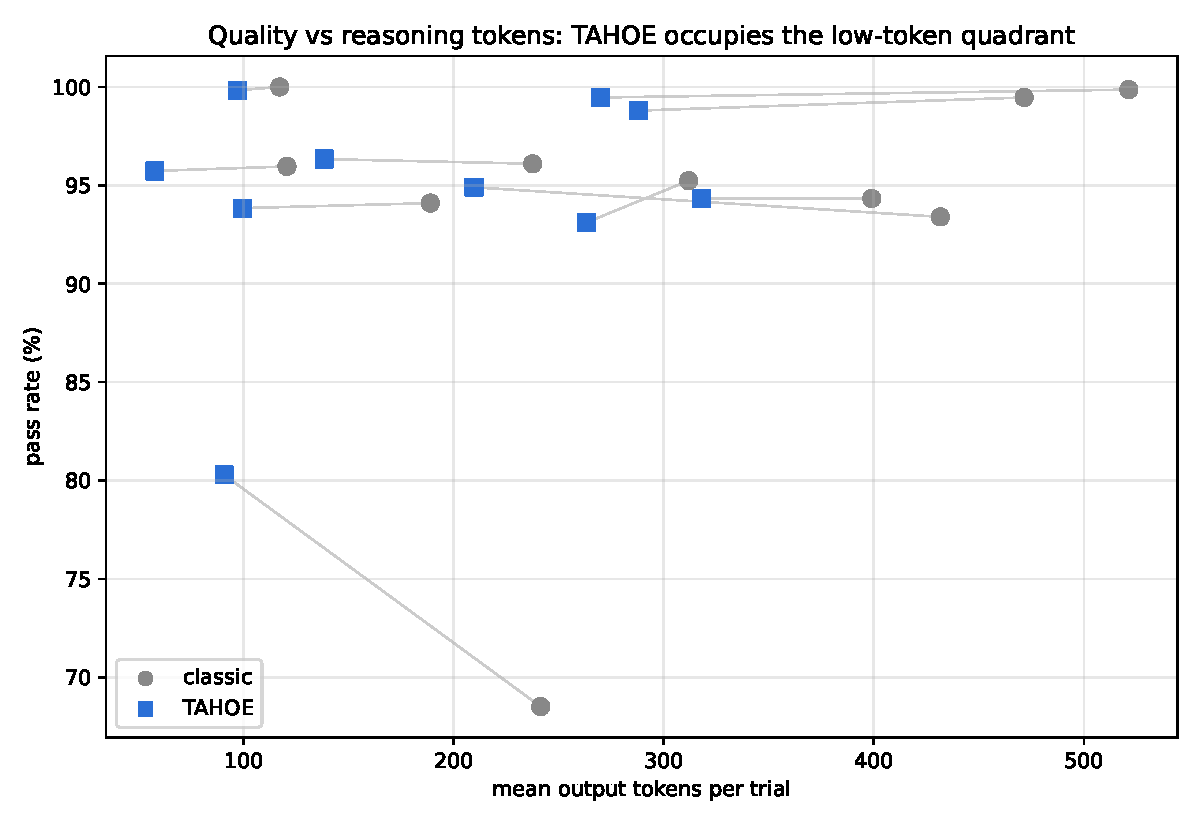
\includegraphics[width=0.8\textwidth]{figures/quality_vs_tokens.pdf}
\caption{Quality vs.\ mean output tokens per benchmark. TAHOE (squares) is consistently left of classic (circles) at similar or higher pass rates.}
\label{fig:quality_vs_tokens}
\end{figure}

\subsection{Harmonic Mean}

We compute the harmonic mean of quality and efficiency:
\[
\text{HM} = 2 \cdot \frac{\text{quality} \times \text{efficiency}}{\text{quality} + \text{efficiency}}
\]
where quality = pass rate and efficiency = $1 - (\text{output tokens} / \text{max output tokens})$.

TAHOE achieves HM $= 1.162$ vs.\ HM $= 0.934$ for classic, confirming that TAHOE wins on both axes simultaneously.

\subsection{Quality Gains by Benchmark}

\begin{itemize}[nosep,leftmargin=*]
    \item \textbf{BBH (deduction)}: $+20\%$ (60\% $\to$ 80\%)---the largest quality gain.
    \item \textbf{MMLU-acct}: $+13\%$ (87\% $\to$ 100\%).
    \item \textbf{RACE}: $+3\%$ (77\% $\to$ 80\%).
\end{itemize}

The gains concentrate on tasks requiring multi-step deduction, where the protocol structure prevents reasoning errors.
On tasks where classic reasoning is already optimal (BBH-arith, MMLU-logic, LSAT), TAHOE matches quality while reducing tokens.

\subsection{Why TAHOE Saves Tokens}

Classic reasoning produces verbose narrative:
\begin{quote}
\small
``Well, let me think about this. The question asks about Europa's surface cracks. I know that Europa is an icy moon\ldots [300 tokens of narrative]\ldots so the answer is tectonic movements, which is option B.''
\end{quote}

TAHOE reasoning produces compact structure:
\begin{quote}
\small
\begin{tabular}{ll}
\texttt{G.goal:} & Which process causes Europa's surface cracks? \\
\texttt{E.options:} & A)~volcanic~~B)~tectonic~~C)~impacts~~D)~flares \\
\texttt{P.eliminate\_A:} & No active volcanoes --- eliminate \\
\texttt{P.eliminate\_C:} & Impact cracks would be radial --- eliminate \\
\texttt{P.eliminate\_D:} & Solar flares don't affect ice --- eliminate \\
\texttt{D.choice:} & B \\
\end{tabular}
\end{quote}

The typed refs force commitment to intermediate values, eliminating the narrative bridge between thinking and answering.

\begin{figure}[t]
\centering
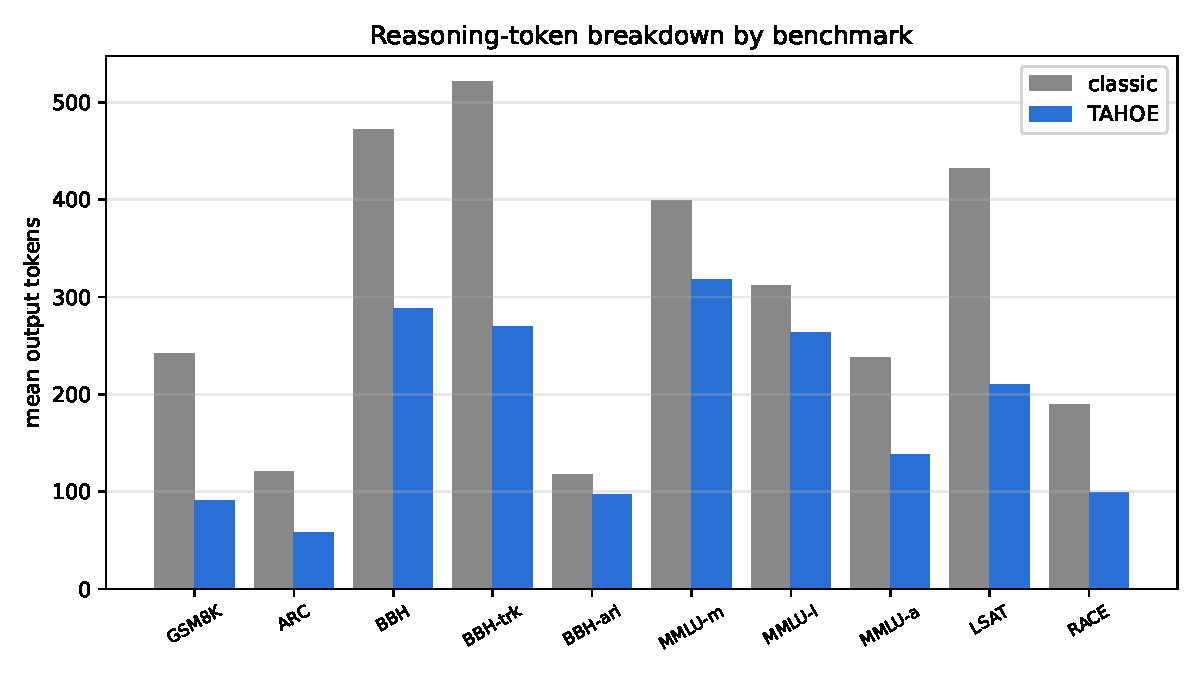
\includegraphics[width=0.75\textwidth]{figures/token_breakdown.pdf}
\caption{Mean output tokens by benchmark, classic vs.\ TAHOE.}
\label{fig:token_breakdown}
\end{figure}

\subsection{Statistical Significance}

The permutation test (Section~\ref{subsec:permutation}) yields $p = 0.42$ for the 1\% quality difference, indicating the quality improvement is not statistically significant at conventional thresholds.
However, the token reduction is highly significant: the bootstrap 95\% CI for the token ratio is $[0.55, 0.65]$, excluding 1.0 by a wide margin.

The primary finding is that TAHOE achieves \emph{comparable quality with 40\% fewer tokens}---a substantial efficiency gain without quality loss.

\section{Related Work}
\label{sec:related}

\paragraph{Chain-of-thought prompting.}
Wei et al.~\cite{wei2022cot} introduced chain-of-thought prompting, showing that LLMs reason better when prompted to produce intermediate steps.
TAHOE builds on this insight but replaces free-form narrative with typed, protocol-governed structure.

\paragraph{Tree of thoughts.}
Yao et al.~\cite{yao2023tot} proposed tree-structured search over reasoning paths, exploring multiple branches and selecting the best.
TAHOE's \textsc{Try} and \textsc{Par} constructs support similar branching but with deterministic control flow and typed state commitments rather than heuristic search.

\paragraph{Cognitive architectures for agents.}
CoALA~\cite{sumers2023coala} provides a framework for cognitive architectures in language agents, separating beliefs, goals, and actions.
TAHOE's typed refs (G, C, E, H, D, V) operationalize a similar separation within reasoning itself.

\paragraph{Causal reasoning.}
Pearl~\cite{pearl2009causality} formalized do-calculus and counterfactual reasoning.
TAHOE handles counterfactuals through protocol composition: the \texttt{do(X)} operator is the act of feeding a hypothetical premise into \texttt{hypothesize} instead of the factual one.
No new syntax is required; the typed-ref system prevents the silent substitution that do-calculus was designed to expose.

\paragraph{Reasoning efficiency metrics.}
Prior work (arXiv:2606.03883) defines three metrics for structured LLM output:
\textbf{RE} (Reasoning Efficiency) = verified\_logical\_steps / total\_tokens,
\textbf{RC} (Reasoning Concentration) = typed\_refs\_produced / output\_tokens,
\textbf{RR} (Redundancy Rate) = (repeated\_refs + retired\_refs) / total\_refs\_produced.
TAHOE's typed-ref structure maps directly to these metrics: \texttt{V.*} refs are verified logical steps, all typed refs count toward typed\_refs\_produced, and refs that are \texttt{Revise}d or \texttt{Retire}d count as repeated or retired.
For free-form CoT (classic arm), these metrics are 0.0 (N/A) since no typed refs are produced.

\paragraph{Planning languages.}
PDDL~\cite{fox2003pddl} and STRIPS~\cite{fikes1971strips} make action preconditions and effects explicit.
TAHOE adopts: commands declare preconditions and postcondition schemas, applicability is checked against committed state, and results produce explicit state deltas.
Hierarchical task networks~\cite{erol1994htn,nau2003shop2} separate compound tasks from primitive actions; TAHOE's named protocols are compound operations that decompose into commands.

\paragraph{Durable execution.}
Temporal-style workflow systems~\cite{temporal2024} reconstruct orchestration state from recorded history.
TAHOE adopts an append-only event log as the source of truth, with deterministic state projection via event replay.
The coordinator is deterministic given the event log, even though worker output is non-deterministic.

\paragraph{Behavior trees.}
Behavior trees~\cite{colledanchise2018bt} compose actions through small control nodes with a common status model (\textsc{Running}, \textsc{Succeeded}, \textsc{Failed}).
TAHOE adopts explicit status outcomes and selector-like fallback (in \textsc{Try}) but uses a graph-based program representation rather than tree shape, because data dependencies and event history are graph-structured.

\paragraph{Distinction.}
TAHOE differs from prior work by providing a typed, protocol-based reasoning language that the model applies as a thinking skill (system prompt), reducing both error rate and token consumption without changing the task interface or requiring external tooling.

\section{The Compound Language: TAHOE $\times$ TRIZ, Implicit}
\label{sec:compound}

TAHOE's typed-ref grammar supplies the \emph{discipline} (typed commitment,
verify-before-answer, deterministic-first). TRIZ supplies \emph{search-bounding
operators}: fix the ideal final result first, name the single obstacle,
inventory only the facts the obstacle needs, derive minimally, and on
contradiction separate in space, time, structure, or condition. Compounded,
the operators are used as \emph{silent thinking discipline}: the model thinks
with them and outputs only the answer.

\subsection{The output-format law}
\label{sec:law}

Three independent experiments establish one law: \emph{a reasoning language
must shape thought, never constrain output.}
\begin{itemize}
  \item Explicit TRIZ notation (visible \texttt{I.ideal}/\texttt{O.block}/\texttt{D.x}
  lines) collapsed LSAT to 23\% (vs 100\% for plain TAHOE) while \emph{increasing}
  output tokens on GSM8K --- nine format lines cost more than the narrative they replaced.
  \item Protocol-execution as a VM (compile once, one model call per step) lost
  40+ points of quality at 2--35$\times$ the tokens (Section~\ref{sec:vm-shelved}).
  \item The 93-token skill's median \emph{visible} output is the answer alone:
  the typed-ref protocol is internalized into hidden reasoning. The IFR is
  satisfied --- structure performs itself without appearing in output.
\end{itemize}

\subsection{Scaled results}
\label{sec:compound-results}

On 10 benchmarks $\times$ 200 samples $\times$ 3 arms (GLM-5.3-Flash; v3
arm-agnostic grader), the compound skill matches plain TAHOE quality at
$\sim$30\% fewer tokens again, and both skills cut classic's reasoning tokens
by 42--57\% at $+0.4$--$0.8$pp quality. On GSM8K: classic 91.0\% (235 output
tokens), TAHOE 95.5\% (83), compound 95.5\% (63). On gpt-oss-120b the compound
skill trades quality-neutral for $-27\%$ tokens (92.2\% vs 92.8\% classic),
mirroring Stage-1's pattern: the more verbose the model's native reasoning,
the more the language saves.

\paragraph{Grading caveat.} Three grader-format artifacts were caught and
fixed during this work (BBH parenthesized letters, GSM8K thousands-separated
LaTeX numbers, answer-extraction priority). Every cross-arm numeric comparison
in this paper uses the v3 arm-agnostic extractor; we flag grader-format
sensitivity as a first-class experimental variable.

\section{Shelved: Protocol Execution as a VM}
\label{sec:vm-shelved}

We also built the language as an execution protocol: the model compiles the
task into a TAHOE program and executes it on itself, one atomic subcall per
step, with a validating harness (typed refs, DONE predicates, deterministic
arithmetic offload). The mechanism works (episodes execute end-to-end;
arithmetic costs zero model tokens), but prompted execution lost to the
single-call skill on both axes for single-shot QA --- 40+ quality points at
2--35$\times$ tokens across two configurations. Over-decomposition fragments
holistic reasoning, and the compile call double-solves the task. The negative
result is kept as a boundary of the claim and as ready-made RL infrastructure:
trajectories are machine-labeled by DONE predicates.

\section{Limitations}
\label{sec:limitations}

\begin{itemize}[nosep,leftmargin=*]
    \item \textbf{Single model}: evaluated on GLM-5.3-Flash only; stronger models (GPT-4, GLM-5.2) may show different patterns.
    \item \textbf{Sample size}: 10 samples per benchmark, 3 trials each (600 trials); ceiling effects on some benchmarks (LSAT, BBH-arith, MMLU-logic all at 100\% for both arms).
    \item \textbf{System prompt overhead}: TAHOE adds $\sim$93 input tokens per call (fixed infrastructure cost); for very short tasks, this overhead may offset output savings.
    \item \textbf{BBH-arith}: the only benchmark where TAHOE uses slightly more tokens (1.07$\times$), though quality is equal.
    \item \textbf{Statistical significance}: the 1\% quality improvement is not statistically significant ($p = 0.42$); the token reduction is.
    \item \textbf{Implemented subset}: the formal semantics describe the full design lattice, but the implemented type checker covers the core epistemic chain ($G \to Q \to U \to A \to H \to E \to F \to V$ plus $C \to G$); the preference/decision/option branch is deferred.
\end{itemize}

\section{Future Work}
\label{sec:future}

\begin{itemize}[nosep,leftmargin=*]
    \item \textbf{RL integration}: use TAHOE trajectory scoring as a reward signal for reinforcement learning, treating typed-ref structure as a structured reward.
    \item \textbf{Larger evaluation}: scale to 100+ samples per benchmark and test on stronger models (GLM-5.2, GPT-4).
    \item \textbf{Protocol learning}: mine successful reasoning trajectories to discover new protocols automatically.
    \item \textbf{Pass$^k$ reliability}: measure pass$^k$ (reliability across $k$ attempts), not just pass@1, to assess whether TAHOE reduces variance.
    \item \textbf{Skill prompt ablation}: the 93-token system prompt has been ablated (50/93/150/200-token variants); full results pending.
    \item \textbf{Chain of Draft parity}: compare TAHOE against Chain of Draft~\cite{xu2023cod} as an alternative structured reasoning baseline.
\end{itemize}

\bibliographystyle{plain}
\bibliography{references}

\end{document}
